\documentclass{boi2014-pl}

\usepackage{enumitem}

\renewcommand{\DayNum}{2}
\renewcommand{\TaskCode}{portals}
\renewcommand{\TaskName}{Portale}

\newcommand{\constant}[1]{{\tt #1}}

\begin{document}
    \begin{wrapfigure}[4]{r}{4cm}
        \vspace{-24pt}
		\includegraphics[width=4cm]{\TaskCode.jpeg}
	\end{wrapfigure}

    \emph{You will be baked, and then there will be cake.}

    W labiryncie znajduje się ciasto, a Ty masz na nie ogromną ochotę.
    Masz mapę labiryntu, która jest prostokątną planszą z $R$ wierszami oraz $C$ kolumnami.
    Każda z komórek mapy zawiera jeden z następujących znaków:
    \begin{description}[itemindent=1pt]
    	\item[\constant{\#}] (hasz) oznaczający ścianę,
        \item[\constant{.}] (kropka) oznaczający wolne pole,
        \item[\constant{S}] (wielka litera s) oznaczający wolne pole, w którym się aktualnie znajdujesz,
        \item[\constant{C}] (wielka litera c) oznaczający wolne pole, w którym znajduje się ciasto.
    \end{description}

    Możesz poruszać się jedynie po wolnych polach oraz przechodzić pomiędzy dwoma wolnymi polami,
    jeśli na mapie sąsiadują ze sobą bokami.
    Dodatkowo, prostokątny obszar labiryntu opisany na mapie jest otoczony z zewnątrz przez ściany.

    Aby dobrać się do ciasta szybciej, zaopatrzyłeś się w urządzenie do tworzenia portali od firmy
    Przysłona Nauka\texttrademark{}, której opis działania znajduje się poniżej.
    W dowolnym momencie może ona wystrzelić portal w jednym z czterech kierunków \emph{góra}, \emph{lewo}, \emph{dół}, \emph{prawo}.
    Gdy portal jest wystrzelony w pewnym kierunku, będzie się w nim poruszał, dopóki nie natrafi na ścianę.
    Wtedy pojawi się na ścianie w którą trafił, po tej stronie, w którą uderzył.
    
    Co najwyżej dwa portale mogą istnieć w dowolnym momencie.
    Jeśli dwa portale są już rozmieszczone w labiryncie, jeden z nich (wybrany przez Ciebie), zostanie zniszczony w momencie kolejnego użycia urządzenia.
    Wystrzelenie portalu w kierunku ściany, gdzie już znajduje się inny portal, zastąpi go (po każdej ze stron ściany może znajdować się co najwyżej jeden portal).
    Zauważ, że na jednej ścianie może znajdować się kilka portali, ale na różnych jej stronach.

    Jeśli dwa portale są umieszczone w labiryncie, możesz ich użyć do teleportacji.
    Stojąc przy jednym z portali, możesz pójść w jego kierunku i znaleźć się na polu obok drugiego portalu.
    Zajmuje to tyle samo czasu, co przejście pomiędzy sąsiednimi polami.

    Możesz założyć, że wystrzelenie portalu nie zajmuje czasu, a przemieszczanie się pomiędzy sąsiednimi polami labiryntu oraz teleportacja przy użyciu portali zajmuje jedną jednostkę czasu.

    \Task
    Mając daną mape labiryntu wraz z Twoją pozycją oraz pozycją ciasta, policz najkrótszy czas, w jakim możesz dobrać się do smakołyku.

    \Input
    W pierwszym wierszu wejścia znajdują się dwie liczby: liczba wierszy na mapie $R$ oraz liczba kolumn $C$.
    Kolejnych $R$ wierszy opisuje mapę.
    Każdy z nich zawiera $C$ znaków: \constant{\#}, \constant{.}, \constant{S} oraz \constant{C} (których znaczenie wyjaśnione jest na górze).

    Znaki \constant{S} oraz \constant{C} pojawią się na wejściu każdy dokładnie jeden raz.

    \Output
    Wyjście powinno zawierać jedną liczbę -- najkrótszy czas, w jakim możesz dostać się do ciasta z Twojej pozycji startowej.

    Możesz założyć, że droga do ciasta zawsze istnieje.

    \Example
    \example
    {
        4 4\newline
        .\#.C\newline
        .\#.\#\newline
        ....\newline
        S...
    }
    {
        4
    }
    {
        Jeden z najkrótszych sposobów dojścia do ciasta: 1) zrób krok w prawo, 2) zrób krok w prawo, wystrzel jeden portal do góry i jeden w dół, 3) przejdź przez dolny portal, 4) zrób krok w prawo i zjedz ciasto.

        \begin{center}
            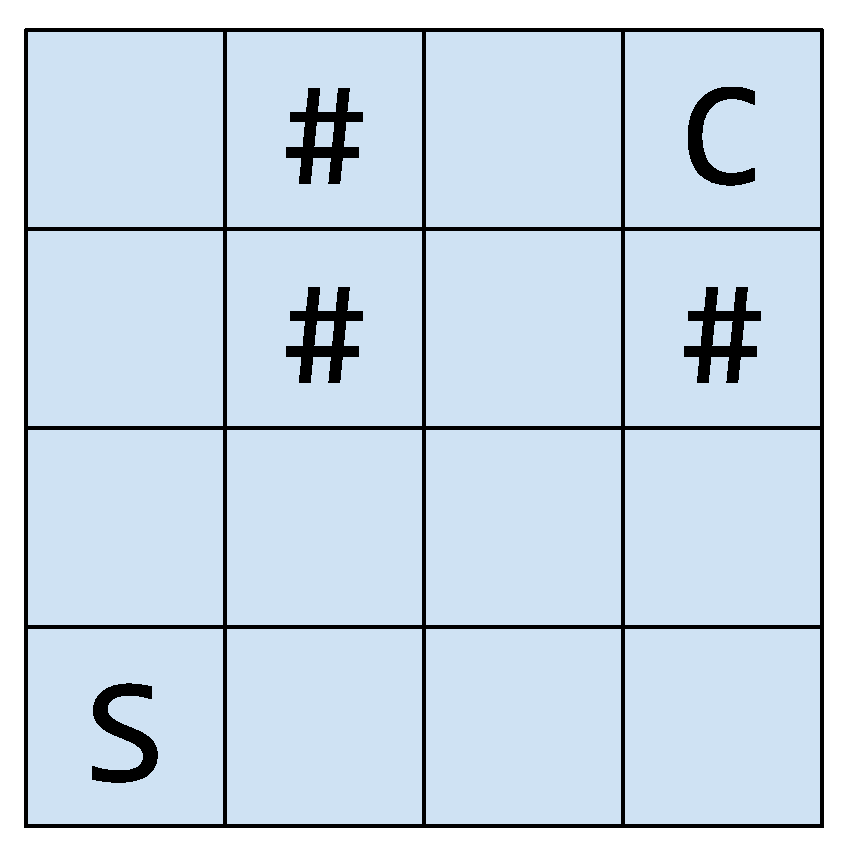
\includegraphics[width=4cm]{portals-example}
        \end{center}
    }

    \Scoring

    \begin{description}[leftmargin=0pt]
        \item[Podzadanie 1 (? punktów):] $0 \le R \le 10, 0 \le C \le 10$.
        \item[Podzadanie 2 (? punktów):] $0 \le R \le 50, 0 \le C \le 50$.
        \item[Podzadanie 3 (? punktów):] $0 \le R \le 200, 0 \le C \le 200$.
        Każde wolne pole ma co najmniej jedną sąsiadującą z nim ścianę.
        \item[Podzadanie 4 (? punktów):] $0 \le R \le 200, 0 \le C \le 200$.
        \item[Podzadanie 5 (? punktów):] $0 \le R \le 1\,000, 0 \le C \le 1\,000$.
    \end{description}

    \Constraints

    \begin{description}
        \item[Limit czasu:] 1 s.
        \item[Dostępna pamięć:] 256 MB.
    \end{description}
\end{document}
